In this section, we will give a more detailed description of previous works
we directly build on and other prerequisites.

\subsection{Optical flow and scene flow}
Let $I_t,I_{t+1} : P \to \mathbb{R}^3$ be two temporally consecutive frames in a
sequence of images.
The optical flow
$\mathbf{w} = (u, v)^T$ from $I_t$ to $I_{t+1}$
maps pixel coordinates in the first frame $I_t$ to pixel coordinates of the
visually corresponding pixel in the second frame $I_{t+1}$,
and can be interpreted as the apparent movement of brightness patterns between the two frames.
Optical flow can be regarded as two-dimensional motion estimation.

Scene flow is the generalization of optical flow to three-dimensional space and additionally
requires estimating depth for each pixel. Generally, stereo input is used for scene flow
to estimate disparity-based depth, however monocular depth estimation with deep networks is also becoming
popular \cite{DeeperDepth, UnsupPoseDepth}.
In this preliminary work, we will assume per-pixel depth to be given.

{
\begin{table}[h]
\centering
\begin{tabular}{llr}
\toprule
\textbf{Output} & \textbf{Layer Operations} & \textbf{Output Dimensions} \\
\midrule\midrule
 & input images $I_t$ and $I_{t+1}$ & H $\times$ W $\times$ 6 \\
\midrule
\multicolumn{3}{c}{\textbf{Encoder}}\\
\midrule
& 7 $\times$ 7 conv, 64, stride 2 & $\tfrac{1}{2}$ H $\times$ $\tfrac{1}{2}$ W $\times$ 64 \\
& 5 $\times$ 5 conv, 128, stride 2 & $\tfrac{1}{4}$ H $\times$ $\tfrac{1}{4}$ W $\times$ 128 \\
& 5 $\times$ 5 conv, 256, stride 2 & $\tfrac{1}{8}$ H $\times$ $\tfrac{1}{8}$ W $\times$ 256 \\
& 3 $\times$ 3 conv, 256 & $\tfrac{1}{8}$ H $\times$ $\tfrac{1}{8}$ W $\times$ 256 \\
& 3 $\times$ 3 conv, 512, stride 2 & $\tfrac{1}{16}$ H $\times$ $\tfrac{1}{16}$ W $\times$ 512 \\
& 3 $\times$ 3 conv, 512 & $\tfrac{1}{16}$ H $\times$ $\tfrac{1}{16}$ W $\times$ 512 \\
& 3 $\times$ 3 conv, 512, stride 2 & $\tfrac{1}{32}$ H $\times$ $\tfrac{1}{32}$ W $\times$ 512 \\
& 3 $\times$ 3 conv, 512, & $\tfrac{1}{32}$ H $\times$ $\tfrac{1}{32}$ W $\times$ 512 \\
& 3 $\times$ 3 conv, 1024, stride 2 & $\tfrac{1}{64}$ H $\times$ $\tfrac{1}{64}$ W $\times$ 1024 \\
\midrule
\multicolumn{3}{c}{\textbf{Refinement}}\\
\midrule
& 5 $\times$ 5 deconv, 512, stride 2 & $\tfrac{1}{32}$ H $\times$ $\tfrac{1}{32}$ W $\times$ 512 \\
\multicolumn{3}{c}{...}\\
\midrule
flow & $\times$ 2 bilinear upsample & H $\times$ W $\times$ 2 \\
\bottomrule
\end{tabular}
\caption {
Overview of the FlowNetS \cite{FlowNet} architecture. Transpose convolutions (deconvolutions)
are used for refinement.
}
\label{table:flownets}
\end{table}
}

\subsection{CNNs for dense motion estimation}
Deep convolutional neural network (CNN) architectures
\cite{ImageNetCNN, VGGNet, ResNet}
became widely popular through numerous successes in classification and recognition tasks.
The general structure of a CNN consists of a convolutional encoder, which
learns a spatially compressed, wide (in the number of channels) representation of the input image,
and a fully-connected prediction network on top of the encoder.

The compressed representations learned by CNNs of these categories do not, however, allow
for prediction of high-resolution output, as spatial detail is lost through sequential applications
of pooling or strides.
Thus, networks for dense prediction introduce a convolutional decoder on top of the representation encoder,
performing upsampling of the compressed features and resulting in a encoder-decoder pyramid.
The most popular deep networks of this kind for end-to-end optical flow prediction
are variants of the FlowNet family \cite{FlowNet, FlowNet2},
which was recently extended to scene flow estimation \cite{SceneFlowDataset}.
Table \ref{table:flownets} gives an overview of the classical FlowNetS architecture for optical flow prediction.

Note that the network itself is a rather generic autoencoder and is specialized for optical flow only through being trained
with supervision from dense optical flow ground truth.
Potentially, the same network could also be used for semantic segmentation if
the number of final and intermediate output channels was adapted from two to the number of classes.
Still, FlowNetS demonstrates that a generic deep encoder-decoder CNN can learn to perform image matching arguably well,
given just two consecutive frames as input and a large enough receptive field at the outputs to cover the displacements.
Note that the maximum displacement that can be correctly estimated depends on the number of strided 2D convolutions (and the stride they use) and pooling
operations in the encoder.
Recently, other, similarly generic,
encoder-decoder CNNs have been applied to optical flow prediction as well \cite{DenseNetDenseFlow}.

\subsection{SfM-Net}
Table \ref{table:sfmnet} shows the SfM-Net \cite{SfmNet} architecture we described
in the introduction.
Motions and full-image masks for a fixed number N$_{motions}$ of independent objects
are predicted in addition to a depth map, and a unsupervised re-projection loss based on
image brightness differences penalizes the predictions.

{
\begin{table}[h]
\centering
\begin{tabular}{llr}
\toprule
\textbf{Output} & \textbf{Layer Operations} & \textbf{Output Dimensions} \\
\midrule\midrule
\multicolumn{3}{c}{\textbf{Conv-Deconv}}\\
\midrule
\multicolumn{3}{c}{\textbf{Motion Network}}\\
\midrule
 & input images $I_t$ and $I_{t+1}$ & H $\times$ W $\times$ 6 \\
 & Conv-Deconv & H $\times$ W $\times$ 32 \\
masks & 1 $\times$1 conv, N$_{motions}$ & H $\times$ W $\times$ N$_{motions}$ \\
FC & From bottleneck: $\begin{bmatrix}\textrm{fully connected}, 512\end{bmatrix}$ $\times$ 2 & 1 $\times$ 512 \\
object motions & fully connected, $N_{motions} \cdot$ 9 & H $\times$ W $\times$ $N_{motions} \cdot$ 9 \\
camera motion & From FC: $\times$ 2 & H $\times$ W $\times$ 6 \\
\midrule
\multicolumn{3}{c}{\textbf{Structure Network}}\\
\midrule
& input image $I_t$ & H $\times$ W $\times$ 3 \\
& Conv-Deconv & H $\times$ W $\times$ 32 \\
depth & 1 $\times$1 conv, 1  & H $\times$ W $\times$ 1 \\
\bottomrule


\end{tabular}

\caption {
SfM-Net \cite{SfmNet} architecture. Here, Conv-Deconv is a simple fully-convolutional
encoder-decoder network, where convolutions and deconvolutions with stride 2 are
used for downsampling and upsampling, respectively. The stride at the bottleneck
with respect to the input image is 32.
The Conv-Deconv weights for the structure and motion networks are not shared,
and N$_{motions} = 3$.
}
\label{table:sfmnet}
\end{table}
}

\subsection{ResNet}
\label{ssec:resnet}
ResNet (Residual Network) \cite{ResNet} was initially introduced as a CNN for image classification, but
became popular as basic building block of many deep network architectures for a variety
of different tasks. Figure \ref{figure:bottleneck}
shows the fundamental building block of ResNet. The additive \emph{residual unit} enables the training
of very deep networks without the gradients becoming too small as the distance
from the output layer increases.

In Table \ref{table:resnet}, we show the ResNet variant
that will serve as the basic CNN backbone of our networks, and
is also used in many other region-based convolutional networks.
The initial image data is always passed through the ResNet backbone as a first step to
bootstrap the complete deep network.
Note that for the Mask R-CNN architectures we describe below, this is equivalent
to the standard ResNet-50 backbone. We now introduce one small extension that
will be useful for our Motion R-CNN network.
In ResNet-50, the C$_5$ bottleneck has a stride of 32 with respect to the
input image resolution. In FlowNetS \cite{FlowNet}, their bottleneck stride is 64.
For accurately estimating motions corresponding to larger pixel displacements, a larger
stride may be important.
Thus, we add a additional C$_6$ block to be used in the Motion R-CNN ResNet variants
to increase the bottleneck stride to 64, following FlowNetS.


{
\begin{table}[h]
\centering
\begin{tabular}{llr}
\toprule
\textbf{Output} & \textbf{Layer Operations} & \textbf{Output Dimensions} \\
\midrule\midrule
 & input image & H $\times$ W $\times$ C \\
\midrule
\multicolumn{3}{c}{\textbf{ResNet}}\\
\midrule
C$_1$ & 7 $\times$ 7 conv, 64, stride 2 & $\tfrac{1}{2}$ H $\times$ $\tfrac{1}{2}$ W $\times$ 64 \\
\midrule
& 3 $\times$ 3 max pool, stride 2 & $\tfrac{1}{4}$ H $\times$ $\tfrac{1}{4}$ W $\times$ 64 \\
\midrule
C$_2$ &
$\begin{bmatrix}
1 \times 1, 64 \\
3 \times 3, 64 \\
1 \times 1, 256 \\
\end{bmatrix}_b$ $\times$ 3
& $\tfrac{1}{4}$ H $\times$ $\tfrac{1}{4}$ W $\times$ 256 \\
\midrule
C$_3$ &
$\begin{bmatrix}
1 \times 1, 128 \\
3 \times 3, 128 \\
1 \times 1, 512 \\
\end{bmatrix}_{b/2}$ $\times$ 4
& $\tfrac{1}{8}$ H $\times$ $\tfrac{1}{8}$ W $\times$ 512 \\
\midrule
C$_4$ &
$\begin{bmatrix}
1 \times 1, 256 \\
3 \times 3, 256 \\
1 \times 1, 1024 \\
\end{bmatrix}_{b/2}$ $\times$ 6
& $\tfrac{1}{16}$ H $\times$ $\tfrac{1}{16}$ W $\times$ 1024 \\
\midrule
C$_5$ &
$\begin{bmatrix}
1 \times 1, 512 \\
3 \times 3, 512 \\
1 \times 1, 2048 \\
\end{bmatrix}_{b/2}$ $\times$ 3
& $\tfrac{1}{32}$ H $\times$ $\tfrac{1}{32}$ W $\times$ 2048 \\
\midrule
C$_6$ &
$\begin{bmatrix}
1 \times 1, 512 \\
3 \times 3, 512 \\
1 \times 1, 2048 \\
\end{bmatrix}_{b/2}$ $\times$ 2
& $\tfrac{1}{64}$ H $\times$ $\tfrac{1}{64}$ W $\times$ 2048 \\

\bottomrule
\end{tabular}
\caption {
Backbone architecture based on ResNet-50 \cite{ResNet}.
Operations enclosed in a []$_b$ block make up a single ResNet \enquote{bottleneck}
block (see Figure \ref{figure:bottleneck}). If the block is denoted as []$_b/2$,
the first convolution operation in the block has a stride of 2. Note that the stride
is only applied to the first block, but not to repeated blocks.
Batch normalization \cite{BN} is used after every residual unit.
}
\label{table:resnet}
\end{table}
}

\begin{figure}[t]
  \centering
  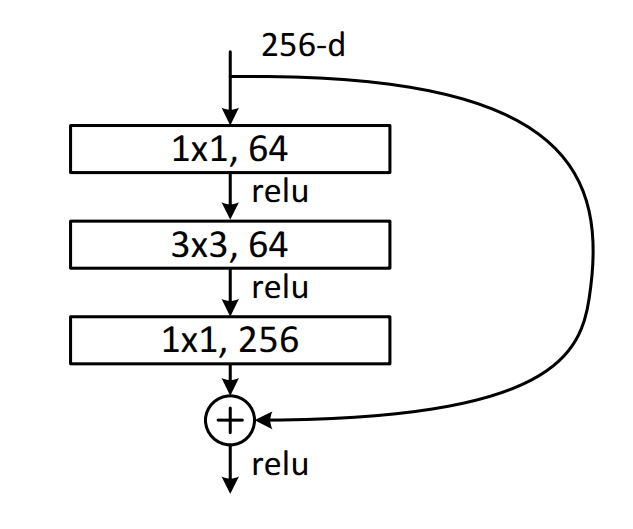
\includegraphics[width=0.3\textwidth]{figures/bottleneck}
\caption{
ResNet \cite{ResNet} \enquote{bottleneck} convolutional block introduced to reduce computational
complexity in deeper network variants, shown here with 256 input and output channels.
Figure taken from \cite{ResNet}.
}
\label{figure:bottleneck}
\end{figure}

\subsection{Region-based CNNs}
\label{ssec:rcnn}
We now give an overview of region-based convolutional networks, which are currently by far the
most popular deep networks for object detection, and have recently also been applied to instance segmentation.

\paragraph{R-CNN}
Region-based convolutional networks (R-CNNs) \cite{RCNN} use a non-learned algorithm external to a standard encoder CNN
for computing \emph{region proposals} in the shape of 2D bounding boxes, which represent regions that may contain an object.
For each of the region proposals, the input image is cropped using the region bounding box and the crop is
passed through the CNN, which performs classification of the object (or non-object, if the region shows background).

\paragraph{Fast R-CNN}
The original R-CNN involves computing one forward pass of the CNN for each of the region proposals,
which is costly, as there is generally a large number of proposals.
Fast R-CNN \cite{FastRCNN} significantly reduces computation by performing only a single forward pass with the whole image
as input to the CNN (compared to the sequential input of crops in the case of R-CNN).
Then, fixed size (H $\times$ W) feature maps are extracted from the compressed feature map of the image,
each corresponding to one of the proposal bounding boxes.
The extracted per-RoI (region of interest) feature maps are collected into a batch and passed into a small Fast R-CNN
\emph{head} network, which performs classification and prediction of refined boxes for all regions in one forward pass.
The extraction technique is called \emph{RoI pooling}. In RoI pooling, the RoI bounding box window over the full image features
is divided into a H $\times$ W grid of cells. For each cell, the values of the underlying
full-image feature map are max-pooled to yield the output value at the cell.
Thus, given region proposals, all computation is reduced to a single pass through the complete network,
speeding up the system by two orders of magnitude at inference time and one order of magnitude
at training time.

{
\begin{table}[t]
\centering
\begin{tabular}{llr}
\toprule
\textbf{Output} & \textbf{Layer Operations} & \textbf{Output Dimensions} \\
\midrule\midrule
& input image & H $\times$ W $\times$ C \\
\midrule
C$_4$ & ResNet \{up to C$_4$\} (Table \ref{table:resnet})  & $\tfrac{1}{16}$ H $\times$ $\tfrac{1}{16}$ W $\times$ 1024 \\
\midrule
\multicolumn{3}{c}{\textbf{Region Proposal Network (RPN)}}\\
\midrule
R$_0$ & From C$_4$: 1 $\times$ 1 conv, 512 & $\tfrac{1}{16}$ H $\times$ $\tfrac{1}{16}$ W $\times$ 512 \\
& 1 $\times$ 1 conv, 4 & $\tfrac{1}{16}$ H $\times$ $\tfrac{1}{16}$ W $\times$ $N_a \cdot$ 4 \\
& flatten & A $\times$ 4 \\
boxes$_{\mathrm{RPN}}$ & decode bounding boxes (Eq. \ref{eq:pred_bounding_box}) & A $\times$ 4\\
& From R$_0$: 1 $\times$ 1 conv, 2 & $\tfrac{1}{16}$ H $\times$ $\tfrac{1}{16}$ W $\times$ $N_a \cdot$ 2 \\
& flatten & A $\times$ 2 \\
scores$_{\mathrm{RPN}}$& softmax & A $\times$ 2 \\
ROI$_{\mathrm{RPN}}$ & sample boxes$_{\mathrm{RPN}}$ and scores$_{\mathrm{RPN}}$ & N$_{RoI}$ $\times$ 6 \\
\midrule
\multicolumn{3}{c}{\textbf{RoI Head}}\\
\midrule
& From C$_4$ with ROI$_{\mathrm{RPN}}$: RoI extraction & N$_{RoI}$ $\times$ 7 $\times$ 7 $\times$ 1024 \\
R$_1$& ResNet \{C$_5$ without stride\} (Table \ref{table:resnet})  & N$_{RoI}$ $\times$ 7 $\times$ 7 $\times$ 2048 \\
ave & average pool & N$_{RoI}$ $\times$ 2048 \\
& From ave: fully connected, N$_{cls}$ $\cdot$ 4 & N$_{RoI}$ $\times$ N$_{cls}$ $\cdot$ 4\\
boxes & decode bounding boxes (Eq. \ref{eq:pred_bounding_box}) & N$_{RoI}$ $\times$ N$_{cls}$ $\cdot$ 4\\
& From ave: fully connected, N$_{cls}$ & N$_{RoI}$ $\times$ N$_{cls}$ \\
classes& softmax, N$_{cls}$ & N$_{RoI}$ $\times$ N$_{cls}$ \\
\midrule
\multicolumn{3}{c}{\textbf{RoI Head: Masks}}\\
\midrule
M$_0$ & From R$_1$: 2 $\times$ 2 deconv, 256, stride 2 & N$_{RoI}$ $\times$ 14 $\times$ 14 $\times$ 256 \\
& 1 $\times$ 1 conv, N$_{cls}$ & N$_{RoI}$ $\times$ 14 $\times$ 14 $\times$ N$_{cls}$ \\
masks & sigmoid & N$_{RoI}$ $\times$ 28 $\times$ 28 $\times$ N$_{cls}$ \\

\bottomrule
\end{tabular}
\caption {
Mask R-CNN \cite{MaskRCNN} ResNet-50 \cite{ResNet} architecture.
Note that this is equivalent to the Faster R-CNN ResNet-50 architecture if the mask
head is left out. In Mask R-CNN, bilinear sampling is used for RoI extraction,
whereas Faster R-CNN uses RoI pooling.
}
\label{table:maskrcnn_resnet}
\end{table}
}


\paragraph{Faster R-CNN}
After streamlining the CNN components, Fast R-CNN is limited by the speed of the region proposal
algorithm, which has to be run prior to the network passes and makes up a large portion of the total
processing time.
The Faster R-CNN object detection system \cite{FasterRCNN} unifies the generation of region proposals and subsequent box refinement and
classification into a single deep network, leading to faster test-time processing when compared to Fast R-CNN
and again, improved accuracy.
This unified network operates in two stages.
In the \emph{first stage}, one forward pass is performed on the \emph{backbone} network,
which is a deep feature encoder CNN with the original image as input.
Next, the \emph{backbone} output features are passed into a small, fully-convolutional \emph{Region Proposal Network (RPN)} head, which
predicts objectness scores and regresses bounding boxes at each of its output positions.
At any of the $h \times w$ output positions of the RPN head,
$N_a$ bounding boxes with their objectness scores are predicted as offsets relative to a fixed set of $N_a$ \emph{anchors} with different
aspect ratios and scales. Thus, there are $N_a \times h \times w$ reference anchors in total.
In Faster R-CNN, $N_a = 9$, with 3 scales, corresponding
to anchor boxes of areas of $\{128^2, 256^2, 512^2\}$ pixels and 3 aspect ratios,
$\{1:2, 1:1, 2:1\}$. For the ResNet Faster R-CNN backbone, we generally have a stride of 16
with respect to the input image at the RPN output (Table \ref{table:maskrcnn_resnet}).

For each RPN prediction at a given position, the objectness score tells us how likely it is to correspond to a detection.
The region proposals can then be obtained as the N highest scoring RPN predictions.

Then, the \emph{second stage} corresponds to the original Fast R-CNN head network, performing classification
and bounding box refinement for each of the region proposals, which are now obtained
from the RPN instead of being pre-computed by an external algorithm.
As in Fast R-CNN, RoI pooling is used to extract one fixed size feature map for each of the region proposals,
and the refined bounding boxes are predicted separately for each object class.

Table~\ref{table:maskrcnn_resnet} includes an overview of the Faster R-CNN ResNet network architecture
(here, the mask head is ignored).

\paragraph{Mask R-CNN}
Faster R-CNN and the earlier systems detect and classify objects at bounding box granularity.
However, it can be helpful to know class and object (instance) membership of all individual pixels,
which generally involves computing a binary mask for each object instance specifying which pixels belong
to that object. This problem is called \emph{instance segmentation}.
Mask R-CNN \cite{MaskRCNN} extends the Faster R-CNN system to instance segmentation by predicting
fixed resolution instance masks within the bounding boxes of each detected object,
which are then bilinearly resized to fit inside the respective bounding boxes.
This is done by simply extending the Faster R-CNN head with multiple convolutions, which
compute a pixel-precise binary mask for each instance.
Note that the per-class masks logits are put through a sigmoid layer, and thus there is no
comptetition between classes in the mask prediction branch.

Additionally, an important technical aspect of Mask R-CNN is the replacement of RoI pooling with
bilinear sampling for extracting the RoI features, which is much more precise.
In the original RoI pooling from Fast R-CNN, the bins for max-pooling are not aligned with the actual pixel
boundary of the bounding box, and thus some detail is lost.

The basic Mask R-CNN ResNet architecture is shown in Table \ref{table:maskrcnn_resnet}.

{
\begin{table}[h]
\centering
\begin{tabular}{llr}
\toprule
\textbf{Output} & \textbf{Layer Operations} & \textbf{Output Dimensions} \\
\midrule\midrule
& input image & H $\times$ W $\times$ C \\
\midrule
C$_5$ & ResNet \{up to C$_5$\} (Table \ref{table:resnet})  & $\tfrac{1}{32}$ H $\times$ $\tfrac{1}{32}$ W $\times$ 1024 \\
\midrule
\multicolumn{3}{c}{\textbf{Feature Pyramid Network (FPN)}}\\
\midrule
P$_5$ & From C$_5$: 1 $\times$ 1 conv, 256 & $\tfrac{1}{32}$ H $\times$ $\tfrac{1}{32}$ W $\times$ 256 \\
P$_4$ & $\begin{bmatrix}\textrm{skip from C$_4$}\end{bmatrix}_p$ & $\tfrac{1}{16}$ H $\times$ $\tfrac{1}{16}$ W $\times$ 256 \\
P$_3$ & $\begin{bmatrix}\textrm{skip from C$_3$}\end{bmatrix}_p$ & $\tfrac{1}{8}$ H $\times$ $\tfrac{1}{8}$ W $\times$ 256 \\
P$_2$ & $\begin{bmatrix}\textrm{skip from C$_2$}\end{bmatrix}_p$ & $\tfrac{1}{4}$ H $\times$ $\tfrac{1}{4}$ W $\times$ 256 \\
P$_6$ & From P$_5$: 2 $\times$ 2 subsample, 256 & $\tfrac{1}{64}$ H $\times$ $\tfrac{1}{64}$ W $\times$ 256 \\
\midrule
\multicolumn{3}{c}{\textbf{Region Proposal Network (RPN)}}\\
\midrule
\multicolumn{3}{c}{$\forall i \in \{2...6\}$}\\
& From P$_i$: 1 $\times$ 1 conv, 512 & $\tfrac{1}{2^i}$ H $\times$ $\tfrac{1}{2^i}$ W $\times$ 512 \\
& 1 $\times$ 1 conv, 6 & $\tfrac{1}{2^i}$ H $\times$ $\tfrac{1}{2^i}$ W $\times$ $N_a \cdot$ 6 \\
RPN$_i$& flatten & A$_i$ $\times$ 6 \\
\midrule
& From \{RPN$_2$ ... RPN$_6$\}: concatenate & A $\times$ 6 \\
& decode bounding boxes (Eq. \ref{eq:pred_bounding_box}) & A $\times$ 6 \\
ROI$_{\mathrm{RPN}}$ & sample bounding boxes \& scores & N$_{RoI}$ $\times$ 6 \\
\midrule
\multicolumn{3}{c}{\textbf{RoI Head}}\\
\midrule
R$_2$ & From \{P$_2$ ... P$_6$\} with ROI$_{\mathrm{RPN}}$: RoI extraction (Eq. \ref{eq:level_assignment}) & N$_{RoI}$ $\times$ 14 $\times$ 14 $\times$ 256 \\
& 2 $\times$ 2 max pool & N$_{RoI}$ $\times$ 7 $\times$ 7 $\times$ 256 \\
F$_1$ & $\begin{bmatrix}\textrm{fully connected}, 1024\end{bmatrix}$ $\times$ 2 & N$_{RoI}$ $\times$ 1024 \\
& From F$_1$: fully connected, N$_{cls}$ $\cdot$ 4 & N$_{RoI}$ $\times$ N$_{cls}$ $\cdot$ 4 \\
boxes & decode bounding boxes (Eq. \ref{eq:pred_bounding_box}) & N$_{RoI}$ $\times$ N$_{cls}$ $\cdot$ 4\\
& From F$_1$: fully connected, N$_{cls}$ & N$_{RoI}$ $\times$ N$_{cls}$ \\
classes& softmax, N$_{cls}$ & N$_{RoI}$ $\times$ N$_{cls}$ \\
\midrule
\multicolumn{3}{c}{\textbf{RoI Head: Masks}}\\
\midrule
M$_1$ & From R$_2$: $\begin{bmatrix}\textrm{3 $\times$ 3 conv} \end{bmatrix}$ $\times$ 4, 256 & N$_{RoI}$ $\times$ 14 $\times$ 14 $\times$ 256 \\
& 2 $\times$ 2 deconv, 256, stride 2 & N$_{RoI}$ $\times$ 28 $\times$ 28 $\times$ 256 \\
& 1 $\times$ 1 conv, N$_{cls}$ & N$_{RoI}$ $\times$ 28 $\times$ 28 $\times$ N$_{cls}$ \\
masks & sigmoid & N$_{RoI}$ $\times$ 28 $\times$ 28 $\times$ N$_{cls}$ \\
\bottomrule
\end{tabular}
\caption {
Mask R-CNN \cite{MaskRCNN} ResNet-50-FPN \cite{ResNet} architecture.
Operations enclosed in a []$_p$ block make up a single FPN
block (see Figure \ref{figure:fpn_block}).
}
\label{table:maskrcnn_resnet_fpn}
\end{table}
}

\paragraph{Feature Pyramid Networks}
In Faster R-CNN, a single feature map is used as the source of all RoI features during RoI extraction, independent
of the size of the bounding box of each RoI.
However, for small objects, the C$_4$ (see Table \ref{table:resnet}) features
might have lost too much spatial information to allow properly predicting the exact bounding
box and a high resolution mask.
As a solution to this, the Feature Pyramid Network (FPN) \cite{FPN} enables features
of an appropriate scale to be used for RoI extraction, depending of the size of the bounding box of an RoI.
For this, a pyramid of feature maps is created on top of the ResNet \cite{ResNet}
encoder by combining bilinearly upsampled feature maps coming from the bottleneck
with lateral skip connections from the encoder (Figure~\ref{figure:fpn_block}).
For each consecutive upsampling block, the lateral skip connections are taken from
the encoder block with the same output resolution as the upsampled features coming
from the bottleneck.

Instead of a single RPN head with anchors at 3 scales and 3 aspect ratios,
the FPN variant has one RPN head after each of the pyramid levels P$_2$ ... P$_6$ (see Table \ref{table:maskrcnn_resnet_fpn}).
At each output position of the resulting RPN pyramid, bounding boxes are predicted
with respect to 3 anchor aspect ratios $\{1:2, 1:1, 2:1\}$ and a single scale ($N_a = 3$).
For P$_2$, P$_3$, P$_4$, P$_5$, P$_6$,
the scale corresponds to anchor bounding boxes of areas $32^2, 64^2, 128^2, 256^2, 512^2$,
respectively.
Note that there is no need for multiple anchor scales per anchor position anymore,
as the RPN heads themselves correspond to different scales.
Now, in the RPN, higher resolution feature maps can be used for regressing smaller
bounding boxes. For example, boxes of area close to $32^2$ are predicted using P$_2$,
which has a stride of $4$ with respect to the input image.
Most importantly, the RoI features can now be extracted at the pyramid level $P_j$ appropriate for a
RoI bounding box with size $h \times w$,
\begin{equation}
j = 2 + j_a,
\end{equation}
where
\begin{equation}
j_a = \mathrm{clip}\left(\left[\log_2\left(\frac{\sqrt{w \cdot h}}{s_0}\right)\right], 0, 4\right)
\label{eq:level_assignment}
\end{equation}
is the index (from small anchor to large anchor) of the corresponding anchor box and
\begin{equation}
s_0 = 256 \cdot 0.125
\label{eq:level_assignment}
\end{equation}
is the scale of the smallest anchor boxes.
This formula is slightly different from the one used in the FPN paper,
as we want to assign the bounding boxes which are at the same scale
as some anchor to the exact same pyramid level from which the RPN of this
anchor is computed. Now, for example, the smallest boxes are cropped from $P_2$,
which is the highest resolution feature map.

The Mask R-CNN ResNet-FPN variant is shown in Table \ref{table:maskrcnn_resnet_fpn}.


\begin{figure}[t]
  \centering
  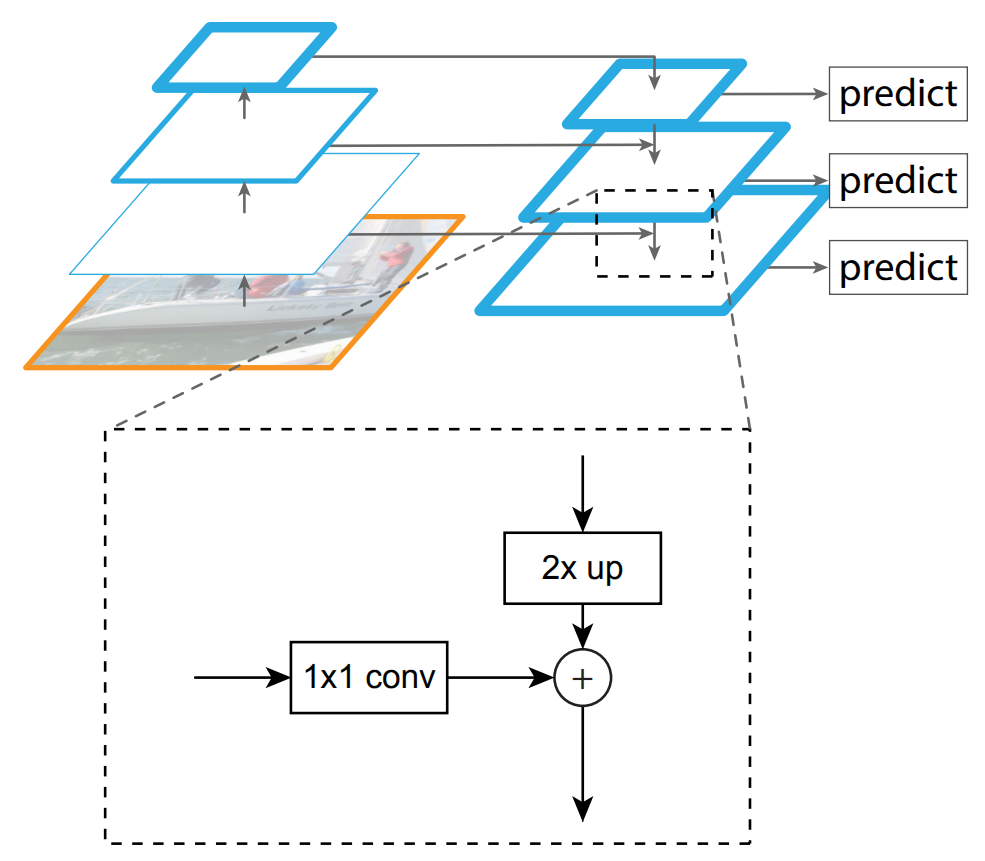
\includegraphics[width=0.3\textwidth]{figures/fpn}
\caption{
FPN block from \cite{FPN}.
Lower resolution features coming from the bottleneck are bilinearly upsampled
and added with higher resolution skip connections from the encoder.
Figure taken from \cite{FPN}.
}
\label{figure:fpn_block}
\end{figure}

\subsection{Mask R-CNN: Training and inference}
\paragraph{Loss definitions}
For regression, we define the smooth-$\ell_1$ regression loss as
\begin{equation}
\ell_{reg}(x) =
\begin{cases}
0.5x^2 &\text{if |x| < 1} \\
|x| - 0.5 &\text{otherwise,}
\end{cases}
\end{equation}
which provides a certain robustness to outliers and will be used
frequently in the following chapters. For vector or tuple arguments, the sum of the componentwise scalar
losses is computed.
For classification with mutually exclusive classes, we define the categorical (softmax) cross-entropy loss,
\begin{equation}
\ell_{cls}(c, c^*) = -\log(),
\end{equation}
where $c^* \in \{0,N_{cls}\}$ is a label (or vector of labels) and $c \in (0,1)$ is the output of a softmax layer. % TODO label has wrong range
Finally, for multi-label classification, we define the binary (sigmoid) cross-entropy loss,
\begin{equation}
\ell_{cls*}(y, y^*) = -y^* \cdot \log(y) - (1 - y^*) \cdot \log(1 - y),
\end{equation}
where $y^* \in \{0,1\}$ is a label (or vector of labels) and $y \in (0,1)$ is the output of a sigmoid layer.

\label{ssec:rcnn_techn}
\paragraph{Bounding box regression}
All bounding boxes predicted by the RoI head or RPN are estimated as offsets
with respect to a reference bounding box. In the case of the RPN,
the reference bounding box is one of the anchors, and refined bounding boxes from the RoI head are
predicted relative to the RPN output bounding boxes.
Let $(x, y, w, h)$ be the top left coordinates, width, and height of the bounding box
to be predicted. Likewise, let $(x^*, y^*, w^*, h^*)$ be the ground truth bounding
box and let $(x_r, y_r, w_r, h_r)$ be the reference bounding box.
The ground truth \emph{box encoding} $b_e^*$ is then defined as
\begin{equation}
b_e^* = (b_x^*, b_y^*, b_w^*, b_h^*),
\end{equation}
where
\begin{equation*}
b_x^* = \frac{x^* - x_r}{w_r},
\qquad
b_y^* = \frac{y^* - y_r}{h_r},
\end{equation*}
\begin{equation*}
b_w^* = \log \left( \frac{w^*}{w_r} \right),
\qquad
b_h^* = \log \left( \frac{h^*}{h_r} \right),
\end{equation*}
which represents the regression target for the bounding box
outputs of the network.

Thus, for each bounding box prediction, the network predicts the box encoding $b_e$,
\begin{equation}
b_e = (b_x, b_y, b_w, b_h),
\end{equation}
where
\begin{equation*}
b_x = \frac{x - x_r}{w_r},
\qquad
b_y = \frac{y - y_r}{h_r},
\end{equation*}
\begin{equation*}
b_w = \log \left( \frac{w}{w_r} \right),
\qquad
b_h = \log \left( \frac{h}{h_r} \right).
\end{equation*}

At test time, to get from a predicted box encoding $b_e$ to the predicted bounding box $b$,
the definitions above can be inverted,
\begin{equation}
b = (x, y, w, h),
\label{eq:pred_bounding_box}
\end{equation}
where
\begin{equation*}
x = b_x \cdot w_r + x_r,
\qquad
y = b_y \cdot b_r + y_r,
\end{equation*}
\begin{equation*}
w = \exp(b_w) \cdot w_r,
\qquad
h = \exp(b_h) \cdot h_r,
\end{equation*}
and thus the bounding box is obtained as the reference bounding box adjusted by
the predicted relative offsets and scales encoded in $b_e$.

\paragraph{Supervision of the RPN}
A positive RPN proposal is defined as one with a IoU of at least $0.7$ with
a ground truth bounding box. For training the RPN, $N_{RPN} = 256$  positive and negative
examples are randomly sampled from the set of all RPN proposals,
with at most $50\%$ positive examples (if there are less positive examples,
more negative examples are used instead).
For examples selected in this way, a regression loss is computed between
predicted and ground truth bounding box encoding, and a classification loss
is computed for the predicted objectness scores.
Specifically, let $s_i^* = 1$ if proposal $i$ is positive and $s_i^* = 0$ if
it is negative, let $s_i$ be the predicted objectness score and $b_i$, $b_i^*$ the
predicted and ground truth bounding box encodings.
Then, the RPN loss is computed as
\begin{equation}
L_{RPN} = L_{obj} + L_{box}^{RPN},
\end{equation}
where
\begin{equation}
L_{obj} = \frac{1}{N_{RPN}} \sum_{i=1}^{N_{RPN}} \ell_{cls}(s_i, s_i^*),
\end{equation}
\begin{equation}
L_{box}^{RPN} = \frac{1}{N_{RPN}^{pos}} \sum_{i=1}^{N_{RPN}} s_i^* \cdot \ell_{reg}(b_i^* - b_i),
\end{equation}
and
\begin{equation}
N_{RPN}^{pos} = \sum_{i=1}^{N_{RPN}} s_i^*
\end{equation}
is the number of positive examples. Note that the bounding box loss is only
active for positive examples, and that the classification loss is computed
between the classes $\{\textrm{object},\textrm{non-object}\}$.

\paragraph{Supervision of the Mask R-CNN RoI head}
For selecting RoIs to train the RoI head network, a foreground example
is defined as one with a IoU of at least $0.5$ with
a ground truth bounding box, and a background example is defined as
one with a maximum IoU in $[0.1, 0.5)$.
A total of 64 (without FPN) or 512 (with FPN) RoIs are sampled, with
at most $25\%$ foreground examples.
Now, let $c_i^*$ be the ground truth object class, where $c_i = 0$
for background examples and $c_i \in \{1, ..., N_{cls}\}$ for foreground examples,
and let $c_i$ be the class prediction.
Then, for any foreground RoI, let $b_i^*$ be the ground truth bounding box encoding and $b_i$
the predicted refined box encoding for class $c_i^*$.
Additionally, for any foreground RoI, let $m_i$ be the predicted $m \times m$ mask for class $c_i^*$
and $m_i^*$ the $m \times m$ mask target with values in $\{0,1\}$, where the mask target is cropped and resized from
the binary ground truth mask using the RPN proposal bounding box.
In our implementation, we use nearest neighbour resizing for resizing the mask
targets.
Then, the ROI loss is computed as
\begin{equation}
L_{RoI} = L_{cls} + L_{box} + L_{mask}
\end{equation}
where
\begin{equation}
L_{cls} = \frac{1}{N_{RoI}} \sum_{i=1}^{N_{RoI}} \ell_{cls}(c_i, c_i^*),
\end{equation}
is the average cross-entropy classification loss,
\begin{equation}
L_{box} = \frac{1}{N_{RoI}^{fg}} \sum_{i=1}^{N_{RoI}} [c_i^* \geq 1] \cdot \ell_{reg}(b_i^* - b_i)
\end{equation}
is the average smooth-$\ell_1$ bounding box regression loss,
\begin{equation}
L_{mask} = \frac{1}{N_{RoI}^{fg}} \sum_{i=1}^{N_{RoI}} [c_i^* \geq 1] \cdot \ell_{cls*}(m_i,m_i^*)
\end{equation}
is the average binary cross-entropy mask loss,
\begin{equation}
N_{RoI}^{fg} = \sum_{i=1}^{N_{RoI}} [c_i^* \geq 1]
\end{equation}
is the number of foreground examples, and
\begin{equation}
[c_i^* \geq 1] =
\begin{cases}
1 &\text{$c_i^* \geq 1$} \\
0 &\text{otherwise}
\end{cases}
\end{equation}
is the Iverson bracket indicator function. Thus, the bounding box and mask
losses are only enabled for the foreground RoIs. Note that the bounding box and mask predictions
for all classes other than $c_i^*$ are not penalized.

\paragraph{Inference}
During inference, the 300 (without FPN) or 1000 (with FPN) highest scoring region proposals
from the RPN are selected. The corresponding features are extracted from the backbone, as during training, by using the RPN bounding boxes,
and passed through the RoI bounding box refinement and classification heads
(but not through the mask head).
After this, non-maximum supression (NMS) is applied to predicted RoIs for which the predicted class is not the background class,
with a maximum IoU of 0.7 of the refined boxes.
Finally, the mask head is applied to the 100 highest scoring (after NMS) refined boxes,
after extracting the corresponding features again.
Thus, during inference, the features for the mask head are extracted using the refined
bounding boxes for the predicted class, instead of the RPN bounding boxes. This is important for not
introducing any misalignment, as the instance masks are to be created inside of the
final, more precise, refined detection bounding boxes.
Furthermore, note that bounding box and mask predictions for all classes but the predicted
class (the highest scoring class) are discarded, and thus the output bounding
box and mask correspond to the highest scoring class.
